\documentclass[utf8]{frontiersSCNS}
\usepackage{gensymb}
\usepackage{url,hyperref,lineno,microtype,subcaption}
\usepackage[onehalfspacing]{setspace}

\linenumbers
\usepackage{wasysym} % provides \DH, \dh, \Thorn, \thorn
% Leave a blank\usepackage{amsmath}
%\DeclareMathOperator{\sign}{sign} line between paragraphs instead of using \\

\usepackage{booktabs}
\usepackage{multirow}
\usepackage{siunitx} %for SI units

\def\keyFont{\fontsize{8}{11}\helveticabold }
\def\firstAuthorLast{Balasubramanian {et~al.}} %use et al only if is more than 1 author
\def\Authors{Suryanarayanan Balasubramanian\,$^{1}$, Roger Waser\,$^{2}$, Martin Hoelzle\,$^{1}$}
\def\Address{$^{1}$University of Fribourg, Department of Geosciences, Fribourg, Switzerland $^{2}$University of
Applied Sciences and Arts, Luzern, Switzerland} \def\corrAuthor{Suryanarayanan Balasubramanian}

\def\corrEmail{suryanarayanan.balasubramanian@unifr.ch}


\begin{document}
\onecolumn
\firstpage{1}

\title[Artificial Ice Reservoirs]{Fountain scheduling for efficient artificial ice reservoirs (Icestupas): theory and
practice }

\author[\firstAuthorLast ]{\Authors}
\address{}
\correspondance{}

\extraAuth{}

% \maketitle

\begin{abstract}
  To sustain productive artificial ice reservoirs (AIRs) with limited water resources requires a high water use
  efficiency (WUE). This can be achieved by the precise scheduling of deficit AIR construction systems taking
  into account the AIRs response to weather and fountain variations. Particularly in the light of climate change
  with rising dependence on this water storage technology, an optimal solution for this task is of paramount
  importance. We solve the corresponding optimization problem, i.e. finding the ideal discharge rate for maximum
  WUE by an approach which offers straightforward application facilities. The automation software uses a
  simplified equation with 6 coefficients that capture the influence of temperature, humidity, wind and solar
  radiation variations on the freezing rate. Historical meteorological data in conjunction with the coordinates,
  altitude and time zone of the site are required to calculate these 6 coefficients. The automated AIR had a WUE
  three times more than the manual AIR. This is a promising result for dry mountain regions, where automated AIR
  technology could scale current mitigation efforts.

	\tiny
	\keyFont{ \section{Keywords:} icestupa, water storage, climate change adaptation, geoengineering, nature based
  solution} %All article types: you may provide up to 8 keywords; at least 5 are mandatory.
\end{abstract}

\section{Introduction}
Climate change adaptation strategies imperatively require a more efficient and sustainable exploitation of water
resources. In arid climates, agriculture depends almost entirely on irrigation and, as glacier meltwater
dwindles, political and economic pressures are being exerted on farmers to increase their water storage
capacity. Thus, a high water use efficiency (WUE) is the prerequisite for a sustainable agricultural production
with limited water resources. 

Automated weather and fountain based scheduling methods are one option for reducing watering volumes for AIR
construction systems and, at the same time, increase WUE.

Proper fountain scheduling requires answers to two questions: (a) When should the water be turned on and off?
(b) How much water should be sprayed? Question (a) can be answered accurately based on the sign of the surface
energy balance. However, question (b) requires information on both the magnitude of the energy balance and the
fountain spray radius over which this energy balance acts.  

\section{Study Sites and data}

\section{Automation software}
The objective of the automation software is to estimate the optimal discharge rate given minimal weather,
fountain and location information. In order to do so, we simplify the methodology used in
\cite{Balasubramanian_2022}. Several assumptions were required to reduce the full energy balance model developed
to a function with minimal variables. We tend to use assumptions that underestimate the associated freezing rate
to optimise for WUE. Below we present each of our assumptions corresponding to the different model modules used
in \cite{Balasubramanian_2022}. 

\subsection{Surface area calculation} \label{sec:shape}

The software approximates the area of the conical AIR to be equal to the area of its circular base. Therefore,
the surface area can be determined using

\begin{equation} A_{cone} =\pi \cdot r_{cone}^2 \label{eq:Area} \end{equation}

Admittedly, this assumption underestimates the surface area of the AIR during the accumulation period and
overestimates the surface area during the ablation period.  

\subsection{Energy balance calculation} \label{sec:energy}

We approximate the energy balance at the surface of an AIR by a one-dimensional description of energy fluxes as
used in \cite{Balasubramanian_2022}:

\begin{equation}
	 q_{freeze} + q_{melt} + q_{T}= q_{SW} + q_{LW} + q_{L} + q_{S} + q_{F} + q_{G}
	\label{eqn:EB}
\end{equation}

Upward and downward fluxes relative to the ice surface are positive and negative, respectively. The first two
terms represent the energy change used for freezing the fountain water and melting the ice respectively. The
third term $q_{T}$ represents the energy used for changing the surface temperature. Here, we define the surface
temperature $T_{ice}$ to be the modelled average temperature of the icestupa surface layer. $q_{SW}$ is the net
shortwave radiation; $q_{LW}$ is the net longwave radiation; $q_{L}$ and $q_{S}$ are the turbulent latent and
sensible heat fluxes. 

The software assumes $T_{ice} = 0 \degree C$ and therefor ignores $q_{T}$, $q_{F}$ and $q_{G}$. All these
assumptions overestimate the freezing energy flux.

\subsubsection{Net Shortwave Radiation \texorpdfstring{$q_{SW}$}{Lg}} \label{sec:SW}

The net shortwave radiation $q_{SW}$ is computed as follows:

\begin{equation} q_{SW} = (1- \alpha_{ice})\cdot SW_{global} \label{eqn:SW} \end{equation}

where $\alpha_{ice}$ is the bare ice albedo value (0.25) and $SW_{global}$ is the global shortwave radiation.
The global shortwave radiation used is modelled using the parametrisation proposed by \cite{Woolf_1968}.

The software ignores (a) the differential absorption of $SW_{direct}$ and $SW_{diffuse}$ due to the conical
shape and (b) the variations in the albedo to simplify the model. Both these assumptions overestimate the solar
radiation thereby underestimating the freezing energy flux.

\subsubsection{Net Longwave Radiation \texorpdfstring{$q_{LW}$}{Lg}} \label{sec:LW}

The net longwave radiation $q_{LW}$ is determined as follows:

\begin{equation}
	q_{LW}= \sigma \cdot \epsilon_a \cdot {(T_a+ 273.15)}^4 -\sigma \cdot \epsilon_{ice} \cdot {(T_{ice}+ 273.15)}^4
	\label{eqn:LW}
\end{equation}

where $T_a$ represents the measured air temperature, $\epsilon_a$ denotes the atmospheric emissivity $T_{ice}$
is the modelled surface temperature given in [$\degree C$], $\sigma=5.67\cdot10^{-8}\,Jm^{-2}s^{-1}K^{-4}$ is
the Stefan-Boltzmann constant and $\epsilon_{ice}$ is the corresponding emissivity value for the Icestupa
surface (0.97).

We approximate the atmospheric emissivity $\epsilon_a$ using the equation suggested by \cite{Brutsaert_1975},
considering air temperature and vapor pressure (Eqn. \ref{eqn:atm_e}). The vapor pressure of air over water and
ice was obtained using Eqn. \ref{eqn:vp}.  

\begin{equation}
	\epsilon_a=1.24 \cdot (\frac{p_{v,w}}{(T_a+273.15)})^{1/7} \label{eqn:atm_e}
\end{equation}

The software assumes $T_{ice} = 0 \degree C$ and ignores the influence of clouds in the atmospheric emissivity.
The first assumption overestimates $q_{LW}$ wherease the seond one underestimates it.  

\subsubsection{Turbulent fluxes} \label{sec:Qs}

The turbulent sensible $q_{S}$ and latent heat $q_{L}$ fluxes are computed with the following expressions
proposed by \cite{Garratt_1992}:

\begin{equation}
	q_{S}= c_{a} \cdot \rho_{a} \cdot p_{a}/p_{0,a} \cdot \frac{\kappa^2 \cdot v_a \cdot
		(T_a-T_{ice})}{{(\ln{\frac{h_{AWS}}{z_{0}}})}^2}
	\label{eqn:qs}
\end{equation}

\begin{equation}
	q_{L}= 0.623 \cdot L_s \cdot \rho_{a}/p_{0,a} \cdot \frac{\kappa^2 \cdot
	v_a(p_{v,w}-p_{v,ice})}{{(\ln{\frac{h_{AWS}}{z_{0}}})}^2}
\end{equation}

where $h_{AWS}$ is the measurement height above the ground surface of the AWS (around $2\,m$ for all sites),
$v_a$ is the wind speed in [$m\,s^{-1}$], $c_a$ is the specific heat of air at constant pressure (1010 J
$kg^{-1} K^{-1}$), $\rho_{a}$ is the air density at standard sea level (1.29 $kg m^{-3}$), $p_{0,a}$ is the air
pressure at standard sea level (1013 $hPa$), $p_{a}$ is the measured air pressure, $\kappa$ is the von Karman
constant (0.4), $z_{0}$ is the surface roughness (3 $mm$) and $L_s$ is the heat of sublimation (2848
$kJ\,kg^{-1}$).  The vapor pressure of air with respect to water ($p_{v,w}$) and with respect to ice
($p_{v,ice}$) was obtained using the formulation given in \cite{huang_2018} :

\begin{equation}
	\begin{split}
		p_{v,w}&=e^{\frac{(34.494 - \frac{4924.99}{T_{a} + 237.1})}{(T_a + 105)^{1.57} \cdot 100}} \cdot \frac{RH}{100} \\
		p_{v,ice}&=e^{\frac{(43.494 - \frac{6545.89}{T_{ice} + 278})}{(T_{ice} + 868)^{2} \cdot 100}} \\
	\end{split} \label{eqn:vp}
\end{equation}

The software ignores the $\mu_{cone}$ parameter thereby underestimating the turbulent fluxes.

\subsection{Automation equation}

Using the above simplifications, we can now approximate $q_{LW}$, $q_{L}$ and $q_{S}$ using just temperature, relative
humidity and wind speed.

Similarly, the diurnal variation of the shortwave radiation can be captured via a gaussian equation. However,
the seasonal variations in the amplitude of the solar radiation are poorly captured by such an equation. Since,
typical AIRs have a construction period spanning less than 3 months, we can ignore the seasonal variations of
solar radiation. Therefore, the net shortwave radiation $q_{SW}$ is computed as follows: 

% The automation equation is composed of two parts namely, (a) linear and (b) gaussian equation. (a)
% approximates the influence of temperature, wind speed and humidity on the expected freezing rate. (b)
% approximates the contribution of solar radiation on the expected freezing rates. 

\begin{subequations}

	\begin{align}
		\label{eq:T}
    \frac{(q_{LW} + q_{S} + q_{L}) \cdot A_{cone} \cdot \Delta t}{L_F} & = a \cdot T_a + b \cdot RH + c \cdot v_a +
  d \\
		\label{eq:SW}
    \frac{q_{SW} \cdot A_{cone} \cdot \Delta t}{L_F} & = \frac{amp}{(\sigma \sqrt{2\pi})} \cdot
    exp\left(\frac{-(time-\mu)^2}{2\sigma^2}\right) \\
		\label{eq:auto}
    \frac{(q_{freeze} + q_{melt}) \cdot A_{cone} \cdot \Delta t}{L_F} & = a \cdot T_a + b \cdot RH + c \cdot v_a + d
  +\frac{amp}{(\sigma \sqrt{2\pi})} \cdot exp\left(\frac{-(time-\mu)^2}{2\sigma^2}\right)
	\end{align}
\end{subequations}

\section{Automation hardware}

\section{Results}

\begin{figure}
	\begin{center}
		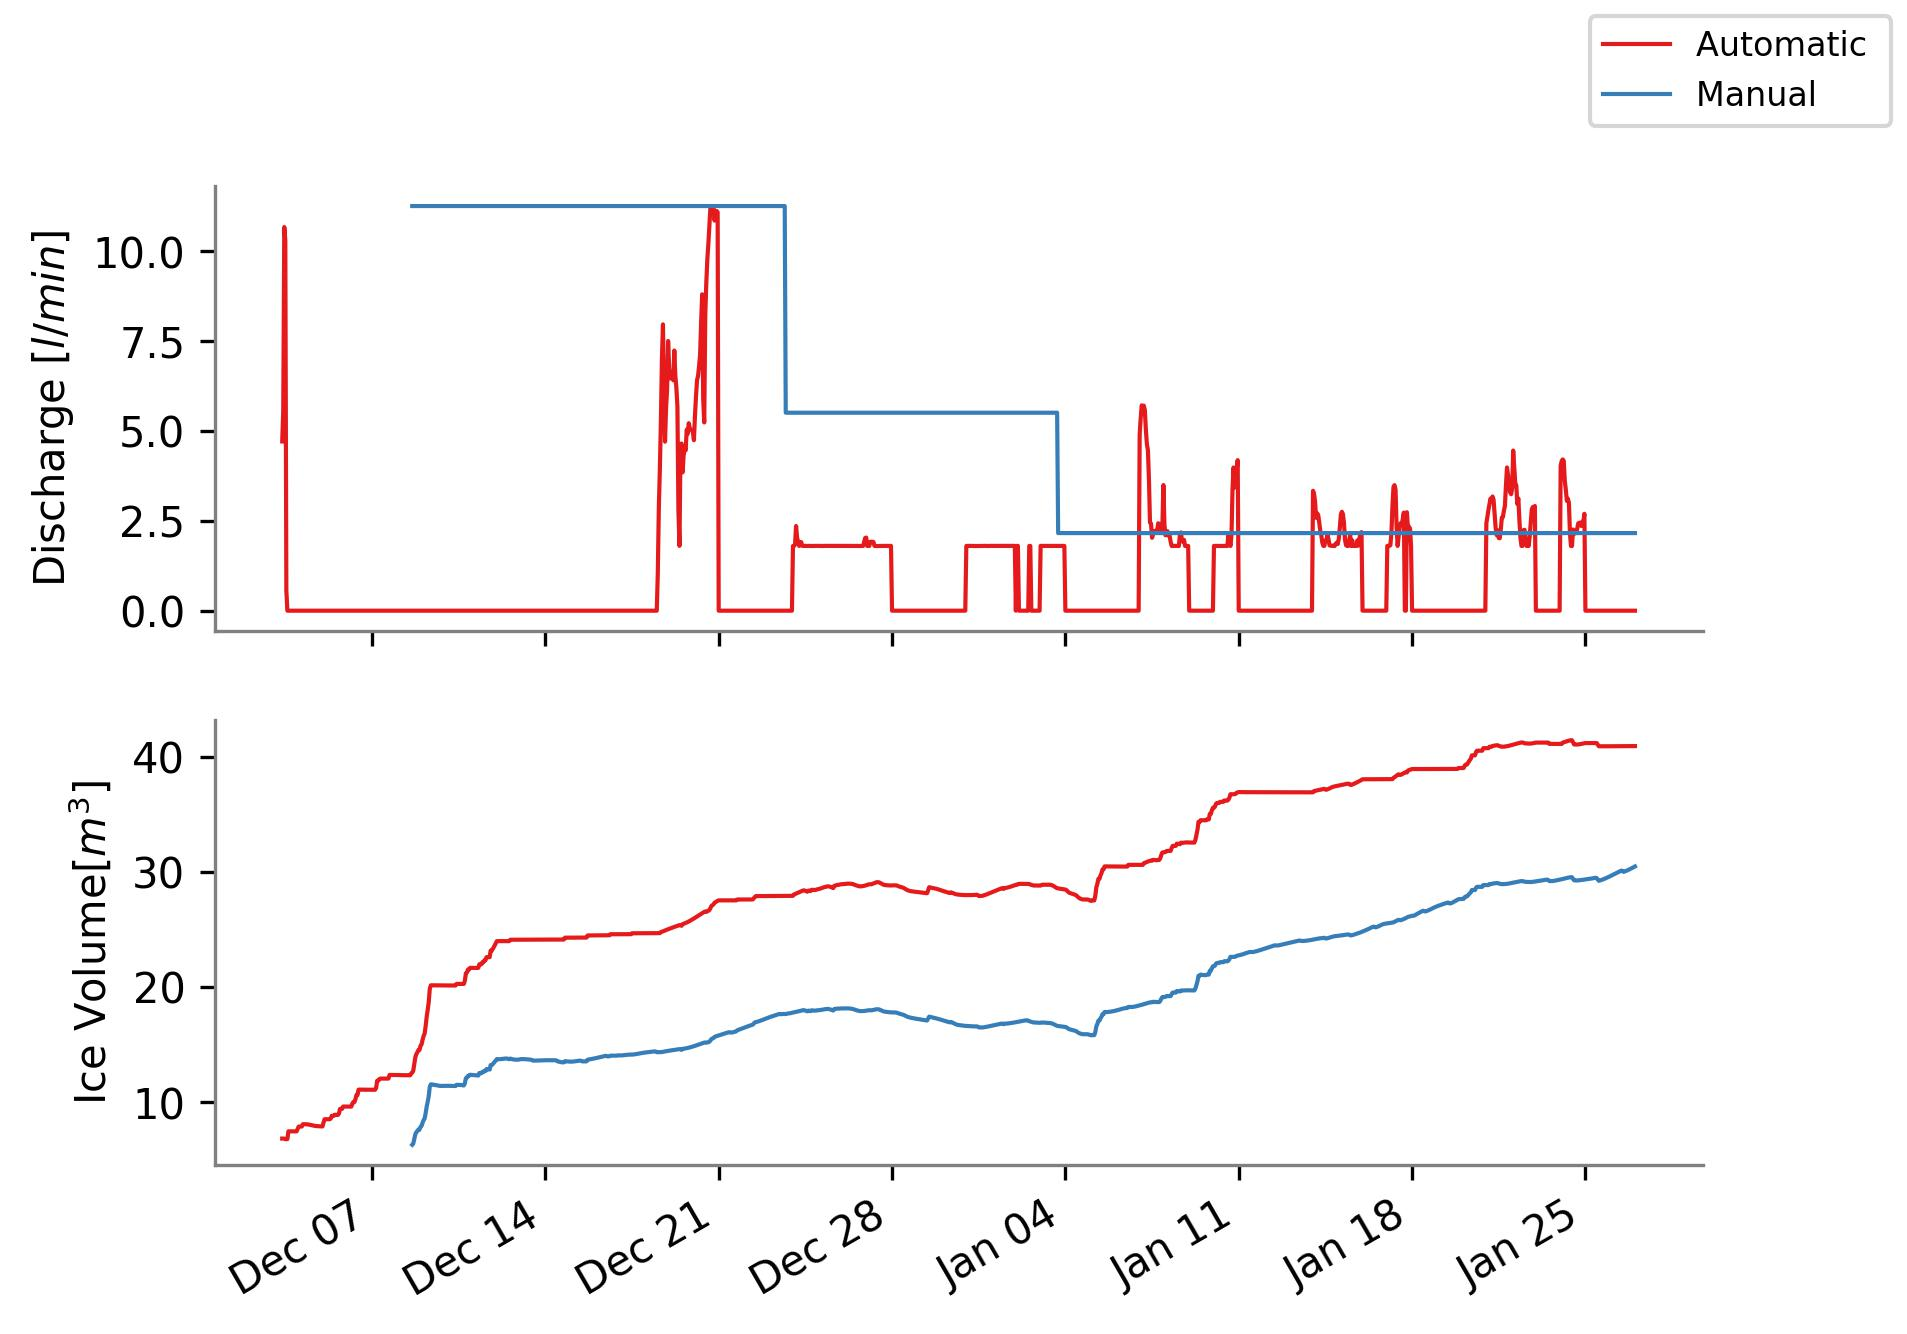
\includegraphics[width=\linewidth]{Figures/autovsmanual.jpg}
	\end{center}
	\caption{Icestupa in Ladakh, India on March 2017 was 24 $m$ tall and contained around 3700 $m^3$
		of water. Picture Credits: Lobzang Dadul}
	\label{fig:old_icestupa}
\end{figure}

\subsection{Validation}

\section{Discussion}

\section{Conclusions}

\section{Appendix}

\bibliographystyle{frontiersinSCNS_ENG_HUMS} \bibliography{refs}

\end{document}
